\documentclass{article}
    \title{\textbf{QuizArt}}
    \author{Lorenzo Camilli, Gaetano Conti, Vincenzo Imperati, Alessio Lucciola}
    \date{24 gennaio 2021}
    	\usepackage{graphicx}
    	\usepackage{hyperref}

\begin{document}

\maketitle

\begin{abstract}
\noindent
App a quiz sui beni culturali italiani, con la possibilità di vincere buoni inerenti.
\end{abstract}

\newpage
\tableofcontents
\newpage

\section{Introduzione}
Stando alle statistiche fornite dall’Istat relative all’anno 2016 (ovvero l’ultimo per il quale sono disponibili i rilevamenti) ben 7 italiani su 10 non si sono mai recati a visitare un museo, eppure l’Italia è la nazione che ha il maggior numero di siti patrimonio dell’umanità riconosciuti dall’UNESCO (in totale 51). Si è stimato che 58,6 milioni di stranieri, solo nel 2018, hanno deciso di visitare il nostro patrimonio museale (46\% del pubblico totale).
\\\indent
Ma quindi noi Italiani non stiamo dando forse, tutto ciò per scontato? Come mai non siamo stimolati a conoscere i nostri beni culturali? Perché questa preziosa eredità non è per noi di fondamentale interesse? La velocità del mondo di oggi ci ha tolto la voglia di passare del tempo davanti a delle opere d’arte? Forse questa pandemia ci ha dato modo e tempo di riflettere sul nostro rapporto con l’immenso patrimonio artistico che la nostra nazione ha da offrire?
\\\indent
Il progetto proposto ha l’obiettivo di riavvicinare gli italiani ai loro beni culturali dandogli il valore che meritano, e tutto questo attraverso un’idea interattiva e ludica. Grazie a QuizArt ci si potrà informare ogni settimana su una tematica differente relativa ai beni culturali italiani, e partecipando al quiz domenicale si potranno vincere visite gratuite, per potersi appassionare sempre di più alla grande ricchezza artistica che il nostro paese ha da offrire.
Sfida i tuoi amici e tutti gli utenti di QuizArt, imparando sempre di più grazie alla magia dell’arte!

\section{Analisi app simili}
L’analisi delle app simili è un’attività necessaria fondamentale per studiare la concorrenza e per capire quali possono essere i punti di forza e di debolezza del nostro prodotto sul mercato.\\\indent
Nel nostro caso abbiamo deciso di analizzare 6 applicazioni competitor, di cui quattro sono giochi a quiz di cultura generale (Trivia Crack, Live Quiz, Quiz senza fine, QuizDuello) e due sono giochi a quiz a tema arte (ArtQ!, Quiz d’arte in italiano). Lo studio svolto è trattato in "Allegato1: Analisi app simili"\cite{Allegato1}.
\\\indent
Durante lo studio di queste app abbiamo trovato diversi spunti utili, anche per analizzare la fattibilità di alcune nostre idee, tra cui:
\begin{itemize}
\item La possibilità di vincita di premi che porta ad un maggiore coinvolgimento degli utenti.
\item Lo sviluppo di un’interfaccia semplice e lineare per aumentare l’usabilità.
\item La possibilità di giocare subito e senza attese.
\item L’inserimento di curiosità tra le domande per diffondere una maggiore consapevolezza artistica negli utenti e spingerli ad interessarsi all’arte intrattenendosi.
\end{itemize}

\section{Needfinding}

\subsection{Interviste}
Nello svolgere le interviste non ci siamo concentrati su un particolare target di persone. Il nostro obiettivo è stato quello di estrapolare più informazioni possibili da potenziali utenti con la speranza di rendere l’applicazione fruibile ad un ampio numero di persone.
\\\indent
Le interviste avevano lo scopo di ragionare sul rapporto tra uomo e arte, e anche su come la pandemia da Covid-19 abbia influenzato questo rapporto. Le nostre prime osservazioni erano sul rapporto stretto tra l’intervistato e i beni culturali, su come esso pianifica, organizza e si informa sui beni culturali che vorrebbe visitare e su cosa dovrebbe cambiare affinché la loro frequenza in questi luoghi aumenti. Le ultime domande invece vertevano sul rapporto dell’intervistato con i giochi a quiz e su come un quiz a tema ‘beni culturali’ potrebbe modificare parzialmente il loro rapporto con essi.
\\\indent
Attraverso l’intervista è stato svolto un importante lavoro di need finding, ed è stato fatto da noi senza avere già in mente cosa stessimo cercando dalle risposte, rimanendo sempre aperti a scoperte impreviste, consapevoli che attraverso l’osservazione si potesse definire il problema. Le interviste erano composte da domande scritte per non influenzare l’opinione degli intervistati e per lasciargli la possibilità di esprimersi in piena libertà, con l’obbiettivo di definire i loro bisogni (need) e non di trovare immediatamente la soluzione ai loro problemi. Le domande sono consultabili in "Allegato2: Domande interviste"\cite{Allegato2}.\\
Il target degli intervistati era composto da 23 persone di cui:
\begin{itemize}
\item 12 maschi e 11 femmine
\item 20 persone in una fascia d’età compresa tra i 18-23 anni
\item 2 over 25
\item 1 over 60
\end{itemize}
Le risposte ottenute dalle interviste sono consultabili in "Allegato3: Risposte interviste"\cite{Allegato3}.\\
I bisogni più importanti emersi nel corso delle interviste sono stati:
\begin{itemize}
\item La possibilità di visitare beni culturali principalmente durante ferie, vacanze o viaggi;
\item L’importanza di informarsi su beni culturali attraverso il web;
\item Il desiderio di pianificare la visita a beni culturali in maniera semplice;
\item La possibilità di essere aggiornato in merito a mostre nella propria zona e/o che trattano categorie artistiche di proprio interesse;
\item La possibilità di voler tornare a visitare beni culturali al termine della pandemia da Covid-19;
\item La possibilità di vincere come premio biglietti e buoni attraverso un quiz a tema ‘beni culturali’ per incentivare il proprio interesse artistico.
\end{itemize}
L'analisi approfondita delle interviste è trattata in "Allegato4: Analisi interviste"\cite{Allegato4}.


\subsection{Questionario}
Il questionario è stato svolto al fine di avere una maggiore consapevolezza sul rapporto tra utente e beni culturali, in modo da poter indirizzare la progettazione dell'applicazione, cercando di avere un confronto più realistico sui need degli utenti. Il questionario ha raggiunto 261 persone, ciò ha garantito uno studio su un pubblico molto eterogeneo.
\\\indent 
La diffusione del questionario è partita il giorno 23/11, a seguito di una fase di verifica tramite questionari pilota al fine di testare le domande e ricercare eventuali errori. La chiusura è avvenuta il giorno 26/11, gran parte del traffico è stato però fatto nelle prime 24 ore di diffusione del questionario.\\
Lo scopo delle domande era:
\begin{itemize}
\item indagare sul rapporto tra beni culturali ed utenti, in particolar modo:
\begin{itemize}
\item la media annuale di visite a beni culturali;
\item le occasioni di visita ai beni culturali;
\item i motivi frenanti nella visita a beni culturali;
\item i mezzi di informazione riguardanti i beni culturali;
\item come il covid-19 ha influenzato il rapporto tra uomo e beni culturali.
\end{itemize}
\item indagare sul rapporto tra giochi a quiz e utenti, e in particolar modo:
\begin{itemize}
\item se ne hanno mai scaricati;
\item perché l’hanno fatto;
\item perché non l’hanno fatto;
\item pensieri su un potenziale gioco a quiz a tema beni culturali.
\end{itemize}
\end{itemize}
Il questionario è consultabile tramite "Allegato5: Domande questionario"\cite{Allegato5}. Se si vuole svolgere il questionario è possibile farlo al seguente link: \href{https://docs.google.com/forms/d/e/1FAIpQLSeiq-80ZoPFimE0_AQif0h2rCf19phYsfOJ1wEj9B0JT0u5WQ/viewform}{Questionario}\\
Le risposte ottenute sono consultabili in "Allegato6: Risposte questionario"\cite{Allegato6}.\\\indent
Tra il campione delle 261 persone che hanno compilato il questionario sono state raggiunte 151 persone (57,9\%) di sesso maschile e 110 persone (42,1\%) di sesso femminile.\\\indent
Dal questionario emergono le seguenti informazioni:
\begin{itemize}
\item la maggior parte degli intervistati visita beni culturali 1-2 volte l’anno
\begin{itemize}
\item principalmente durante le ferie, i weekend e le vacanze.
\end{itemize}
\item i principali mezzi di informazione sui beni culturali sono il web e il passaparola;
\item il Covid ha influenzato molto il rapporto che c’era tra gli utenti e i beni culturali;
\item i motivi frenanti nella visita a beni culturali sono principalmente la mancanza di tempo, la distanza dai beni culturali e il prezzo dei biglietti;
\item la maggior parte degli utenti ha scaricato giochi a quiz, ma quasi mai app a tema artistico;
\item i motivi principali per cui hanno scaricato giochi a quiz sono:
\begin{itemize}
\item bisogno di un passatempo;
\item sfidare gli amici;
\item cultura personale.
\end{itemize}
\end{itemize}
Per visionare un'analisi dettagliata dei dati ottenuti dal questioanrio consultare "Allegato7: Analisi questionario"\cite{Allegato7}.

\section{Tasks}
Una volta raccolti i need abbiamo identificato i task su cui concentrarsi per lo sviluppo dell’app. In particolare, l’analisi generale del questionario ci ha permesso di prendere decisioni decisive sui task. Di seguito un riassunto dell’indice di gradimento di alcune possibili funzionalità dell’applicazione, gli utenti nel questionario:
\begin{itemize}
\item 8.79/10 l’utilità di vincere dei buoni;
\item 8.17/10 l’utilità delle curiosità durante il quiz;
\item 8.06/10 l’utilità della bacheca informativa;
\item 7.92/10 l’utilità dei temi settimanali;
\item 7.13/10 l’utilità dei giochi a quiz per imparare;
\item 6.83/10 l’utilità della classifica tra amici.
\end{itemize}

In base a questi dati abbiamo deciso che i task saranno i seguenti:
\begin{enumerate}
\item Quiz:
	\begin{enumerate}
	\item Quiz Giornaliero;
	\item Quiz Settimanale;
	\end{enumerate}
\item Bacheca Informativa;
\item Shop Buoni.
\end{enumerate}
Di seguito una descrizione dei task (sono sottolieati i need a cui essi rispondono):
\begin{enumerate}
\item Come si può notare dalla lista in alto, il primo task è diviso in due subtask. L’applicazione permette due modalità di gioco, il Quiz giornaliero ed il Quiz Settimanale (\underline{passatempo}). La differenza sostanziale tra i due è che il primo può essere giocato a qualsiasi ora del giorno mentre il secondo si svolge una sola volta a settimana, in un dato giorno e in un dato orario (la data precisa verrà notificata), ed ha la particolarità di essere in diretta con tutti gli utenti che vi stanno partecipando.\\Con Quiz Live si intende che tutti i giocatori giocano allo stesso momento e sullo stesso set di domande (\underline{spirito di competizione}). Entrambe le modalità permettono di guadagnare punti ad ogni risposta corretta, ma nel quiz settimanale si guadagnano molti più punti rispetto a quello giornaliero e per questo vale la pena parteciparvi (\underline{vincita premi}). Ad ogni risposta viene visualizzata una curiosità in modo da apprendere cose nuove. Ogni settimana viene scelto un \underline{tema diverso} e tutte le domande verteranno su quello.
\item Il secondo task prevede una bacheca \underline{informativa}. L’obiettivo della bacheca è di aiutare l’utente nella visita del bene culturale. I beni culturali sono ordinati in ordine crescente in base alla \underline{distanza}. Per ogni bene culturale vengono evidenziati il \underline{tempo di visita}, il \underline{prezzo dei biglietti} ed un breve descrizione.
\item Il terzo task prevede lo shop dei buoni. Giocando, si guadagnano dei punti spendibili all’interno dello shop. Questa sezione permette di convertire i punti in buoni spendibili nei beni culturali convenzionati presenti nella bacheca informativa (\underline{demotivazione prezzo}). Il buono non è altro che un codice, quindi basterà recarsi nel bene culturale che preferiamo, mostrarlo in cassa ed ottenere il biglietto (pagando una differenza nel caso in cui il buono non copra l’intera cifra del biglietto).
\end{enumerate}
   
\section{Storyboarding}
Per ognuno dei task è stato realizzato uno storyboard corrispondente. Gli storyboard prodotti sono visionabili in "Allegato8: Storyboards"\cite{Allegato8}.\\
Qui una rapida descrizione degli scenari delle singole vignette:
\begin{description}
\addtolength{\itemindent}{0.5cm}
\item [Quiz giornaliero] Siamo su un autobus, manca diverso tempo prima dell’arrivo alla nostra fermata, ne approfittiamo per giocare a QuizArt, sbagliamo una risposta all’interno del quiz giornaliero e dall’errore impariamo una nuova cosa.
\item [Quiz settimanale] Siamo su una poltrona, è domenica e sono le 11:59, ci arriva una notifica che il quiz settimanale sta per avere inizio, non vediamo l’ora di giocare dato che questa settimana ci siamo allenati molto sui quiz giornalieri in vista di questo momento.
\item [Bacheca informativa] Siamo appena arrivati nella città di Pisa, entriamo nella bacheca informativa di QuizArt per vedere quali beni culturali abbiamo nelle vicinanze, leggiamo diverse informazioni sulla famosa torre presente a Pisa fremendo dalla voglia di visitarla.
\item [Shop Buoni] Giocando ai quiz presenti in QuizArt ci è venuta voglia di visitare un bene culturale, perciò andiamo nello shop e convertiamo diversi punti in un buono da 20 euro, qualche giorno dopo ci rechiamo in un bene culturale e presentiamo alla cassa il codice del nostro buono per ottenere uno sconto sul biglietto.
\end{description}

\section{Prototyping}
Una volta scelti i task siamo passati alla fase di prototyping. Nel disegnare i prototipi abbiamo utilizzato il “paper prototyping”, un approccio low-fidelity che prevede di disegnare i prototipi su carta.
Abbiamo inoltre utilizzato un approccio iterativo: siamo partiti da un primo prototipo e lo abbiamo via via migliorato fino ad ottenere un risultato soddisfacente.
\\\indent
Partendo dalle specifiche dei task abbiamo iniziato a disegnare una prima versione del sistema. Questa prima versione è servita per renderci conto della reale dimensione del sistema in termini di numero di schermate. Sono stati fatti dei test inter nos e con alcuni utenti (utilizzando il metodo “human computer”) per testare la validità delle interfacce. Sono stati evidenziati numerosi difetti quali la difficoltà nel generare un buono nello shop a causa dell’utilizzo di uno slider, un uso scorretto di alcuni elementi grafici che rendevano difficile la comprensione delle domande e l’implementazione di funzionalità non ancora ben definite come la visualizzazione degli orari di apertura nella bacheca e le informazioni visualizzabili relative a buoni scaduti.
\\\indent
Abbiamo quindi migliorato il prototipo cartaceo andando a risolvere tutti i problemi che avevamo riscontrato e generando una nuova versione dell’applicazione. A causa dell’elevato numero di interfacce nei quiz giornaliero e settimanale, non è stato possibile prototipare tutte le schermate su carta quindi, una volta definita la struttura generale di QuizArt, abbiamo iniziato ad importare tutto il lavoro svolto su Marvel. Questo ci ha permesso di iniziare ad effettuare i test su un'interfaccia molto simile a quella finale. Da questi test sono emersi ulteriori problemi che sono stati via via risolti in iterazioni successive. E’ stata quindi generata una terza versione nonché la versione finale dell’applicazione.
\\\indent
La Versione 1 consiste quindi nei prototipi cartacei, visionabili nella cartella allegata.
\\\indent
La Versione 2 consiste nel primo prototipo in Marvel, visionabili tramite il seguente link: \href{https://marvelapp.com/prototype/bhcf89g/screen/76246379}{Versione 2}.
\\\indent
La Versione 3 consiste nel secondo ed ultimo nonché definitivo prototipo in Marvel, visionabile tramite il seguente link:
\href{https://marvelapp.com/prototype/bhcf89g/screen/75702736}{Versione 3}
\\\indent In "Allegato9: Analisi prototipi"\cite{Allegato9} vengono analizzate le varie versioni dei prototipi. In "Allegato10: Changelog prototipi"\cite{Allegato10} vengono mostrati i cambaiemnti effettuati.

\section{Testing}
Sono stati svolti vari test per valutare le interfacce nelle varie versioni di QuizArt. Nella versione 1 sono stati svolti dei test su un piccolo bacino di utenza e inter nos sfruttando il metodo dello “Human Computer” e lavorando direttamente sui prototipi cartacei.
\\\indent
Una volta importato il progetto su Marvel abbiamo iniziato a svolgere i test sfruttando il suddetto software e presentando agli utenti una interfaccia molto simile a quella finale. I test sulle versioni 2 e 3 sono stati svolti utilizzando il metodo “Think Aloud” quindi facendo commentare agli utenti tutto quello che pensavano e facevano all’interno delle interfacce senza l’aiuto dell’amministratore (a meno di evidenti difficoltà nel proseguire il test). Alla fine, se necessario, sono state poste delle domande integrative in base all’andamento del test.
\\\indent
In "Allegato11: Risultati test"\cite{Allegato11} vengono descritti gli esiti dei test.

\section{Funzionalità definitive}

\paragraph{Quiz giornalieri} possono essere giocati ogni giorno a qualsiasi orario. Ogni partita conta 10 domande con 4 risposte multiple dove solo una di queste è corretta. Ci sono 10 secondi di tempo per rispondere, dopo i quali la domanda verrà conteggiata come errata. Ad ogni risposta corretta verranno assegnati dei punti. I punti ottenibili aumentano ad ogni domanda perciò rispondere correttamente alla prima domanda ti darà meno punti rispetto al rispondere correttamente alla decima. Tra una domanda e l’altra ci sarà sempre una piccola curiosità relativa alla domanda stessa che ti permetterà di ampliare le tue conoscenze. Dal pannello della curiosità, quando sei pronto a passare alla domanda successiva basterà cliccare su “continua”. In qualsiasi momento si può uscire dal quiz cliccando la “X” in alto a sinistra (i punti guadagnati verranno mantenuti).
\\ 
Attenzione, dopo la decima giocata giornaliera potrai continuare a giocare ma non otterrai più punti, per continuare a farlo dovrai ritornare il giorno seguente e ricominciare a giocare;

\paragraph{Quiz settimanali} sono disponibili solo un giorno alla settimana in un dato orario che viene visualizzato nella home (es: la Domenica alle 15). Entro cinque minuti prima dell’orario stabilito potrai unirti alla sala di attesa, visualizzerai un countdown e quando questo arriverà a zero inizierai a giocare. Il funzionamento è simile a quello del quiz giornaliero solo che è live quindi si gioca con tutti i giocatori nello stesso istante e tutti visualizzano la medesima domanda. Anche qui i punti sono incrementali ma valgono 7 volte di più di quelli giornalieri. Hai 10 secondi di tempo per rispondere alla domanda, dopo i quali si visualizza il risultato (se non si risponde la domanda verrà conteggiata come errata). Viene visualizzata la curiosità e dopo 10 secondi si passa automaticamente alla domanda successiva. Se vinci il quiz otterrai un bonus di vittoria pari a sette volte i punti ottenuti da tutte le risposte corrette. In qualsiasi momento si può uscire dal quiz cliccando la “X” in alto a sinistra (i punti guadagnati verranno mantenuti). Attenzione a non perdere il quiz settimanale, se non arrivi in tempo, dovrai attendere la settimana successiva.

\paragraph{Bacheca} in questa sezione dell’app puoi visualizzare tutti i beni culturali convenzionati vicini a te semplicemente accedendovi e attivando il gps. Verrà visualizzata una lista di beni culturali in ordine crescente in base alla distanza. In alto potrebbero comparire ulteriori beni che sponsorizzano l’applicazione. Puoi cliccare su uno di essi per avere varie info sul bene culturale quali:
\begin{itemize}
\item Una descrizione del bene culturale
\item Il prezzo del biglietto per l’ingresso
\item Il tempo di visita medio
\item La posizione del bene culturale (che rimanda a Google Maps)
\item Il sito web del bene culturale (gestito dal browser)
\end{itemize}

\paragraph{Shop} in questa sezione dell’app si potranno convertire i punti guadagnati giocando ai quiz in un buono spendibile nei beni culturali convenzionati. Seleziona il valore che intendi convertire ricordando che 10000 punti equivalgono ad 1 euro e clicca su “converti”. Una volta convertito un buono potrai visualizzarne il codice QR (o testuale) che servirà per utilizzarlo. Se il valore del buono non copre il prezzo del biglietto allora dovrai pagare il saldo rimanente. Se invece il biglietto costa meno del valore del buono, rimarrà del saldo nel buono stesso che potrai riutilizzare in futuro in altri beni culturali. Ricorda che il buono rimane valido per un anno a partire dal giorno in cui è stato generato.
\\\indent
Il buono è utilizzabile in ogni bene culturale convenzionato. Puoi visualizzare tutti i beni convenzionati vicini a te nella sezione “Bacheca” semplicemente accedendovi e attivando il gps. Verrà visualizzata una lista di beni culturali in ordine crescente in base alla distanza. In alto potrebbero comparire ulteriori beni che sponsorizzano l’applicazione. Puoi cliccare su uno di essi per avere varie info sul bene culturale quali prezzo, tempo di visita medio, posizione, sito web, etc.

\section{Studio di fattibilità}
Ci siamo concentrati nello studiare la fattibilità del task riguardante lo shop siccome il sistema di punteggio che permette l'acquisto di buoni é la specifica piú ambiziosa.
\\\indent
L’idea è quella di realizzare una piattaforma simile a 18app. L’utente seleziona il valore che vuole convertire in un buono e viene generato un codice utilizzabile nei centri convenzionati. Si potrà sfruttare il codice QR nel caso in cui il bene culturale disponga di uno scanner, altrimenti il codice si potrà inserire manualmente.
\\\indent
Questo sistema è facilmente implementabile in una applicazione a quiz come QuizArt, gli utenti potranno generare il buono direttamente dall’applicazione.
\\\indent
Un ulteriore problema è che non tutti i beni culturali potrebbero accettare buoni generati da un’applicazione poco conosciuta e senza alcuna garanzia di ottenere il rimborso. Occorre quindi stipulare delle convenzioni con i beni culturali in modo da definire le condizioni e stipulare delle convenzioni. Inoltre, per ottenere ulteriore visibilità (e quindi una maggiore affidabilità), si potrebbe cercare l’aiuto della pubblica amministrazione per sponsorizzare l’applicazione.
\\\indent
Un servizio simile a quello proposto da QuizArt è quello offerto da MilanoGuida che permette di acquistare buoni regalo per visitare più di 500 beni culturali convenzionati in Lombardia, fino all’esaurimento del saldo all’interno del buono. Questo servizio giustifica la fattibilità dello shop nella nostra applicazione.
\\\indent
Per sostenere l'applicazione, si adotterà un sistema di sponsorizzazioni. Ogni bene culturale potrà chiedere a QuizArt di essere sponsorizzato ottenendo una maggiore visibilità nella bacheca. Si potrà inoltre creare un intero set di domande sul bene culturale (o opere al suo interno) in modo da portare gli utenti ad interessarsi.
\\\indent
E’ stato fatto uno studio sulla quantità di punti da assegnare ad ogni domanda. Lo scopo era quello di trovare un giusto equilibrio nei punti guadagnati in base alla bravura dell’utente ed il tempo passato a giocare. Alla fine è stato deciso che 10000 punti corrispondevano ad 1 euro. I punti vengono assegnati in maniera incrementale in base al numero di domanda, ossia il numero di punti guadagnabili è direttamente proporzionale alla difficoltà della domanda. Inoltre, ai punti del quiz settimanale è stato assegnato un fattore moltiplicativo pari a 7 rispetto ai punti del quiz giornaliero.
\\\indent
Qui di seguito è presente le tabelle in cui vengono mostrati i punti guadagnati in ogni domanda:

\begin{figure}[htp]
\begin{center}
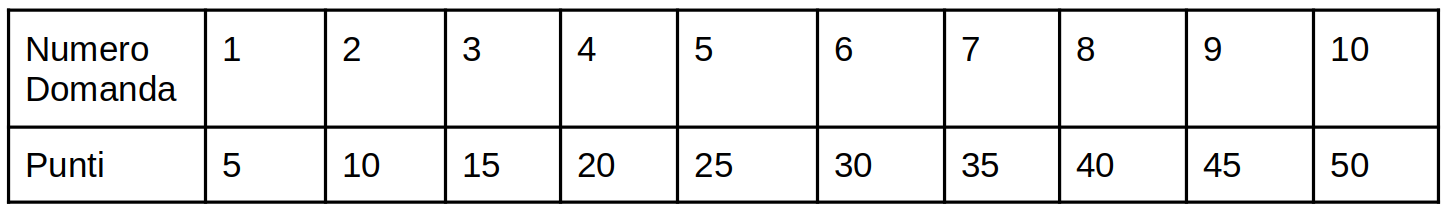
\includegraphics[width=0.75 \textwidth]{tabella giornaliero.png}
\caption{Tabella punteggi quiz giornaliero}
\end{center}
\end{figure}

\begin{figure}[htp]
\begin{center}
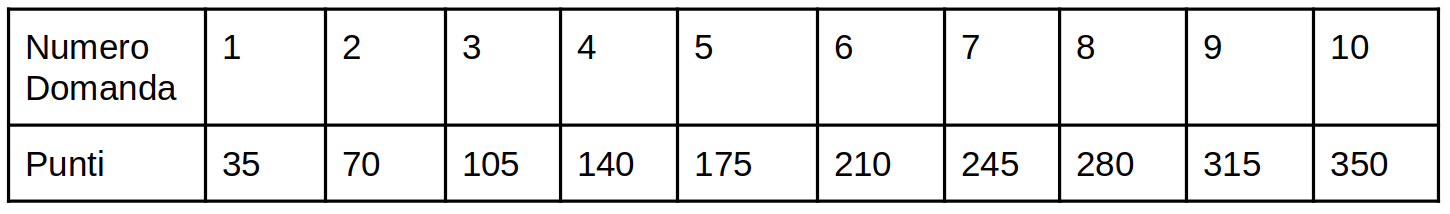
\includegraphics[width=0.75 \textwidth]{tabella settimanale.png}
\caption{Tabella punteggi quiz settimanale}
\end{center}
\end{figure}

Qui di seguito alcune casistiche:
\begin{itemize}
\item Se si indovinano tutte le domande nel quiz giornaliero si ottengono 275 punti;
\item Se si indovinano tutte le domande nel quiz settimanale si ottengono 15400 punti (compreso il bonus vittoria);
\item Se si indovinano tutte e 10 le risposte per la metà dei quiz giornalieri in una settimana si ottengono 275*35 = 9625 punti;
\item Se si indovina una domanda sì e una no in tutti i quiz giornalieri per una settimana si ottengono 150*70 = 10500 punti;
\item Ogni giorno si possono totalizzare al massimo 2750 punti (10 quiz giornalieri con tutte risposte corrette);
\end{itemize}

\section{Conclusioni}
Il progetto ci ha portato ad affrontare gli effettivi problemi dei designer, in particolare quello di interfacciarsi con gli utenti e con la psicologia umana cercando il più possibile di soddisfare le esigenze degli utenti, seguendo tutte le fasi del processo di sviluppo di un'applicazione.
\\\indent
Con il need finding abbiamo dovuto analizzare pensiero umano cercando di capire cosa potrebbe davvero interessare ai possibili utenti, il tutto tramite l’osservazione e il dialogo con essi, ponendo domande che siano mirate e da cui possano scaturire riflessioni e idee, facendo ipotesi e cercando smentite o conferme (questionari), con il fine di capire come poter aiutare l’utente a svolgere il compito che ci siamo prefissati. Successivamente abbiamo dovuto immedesimarci nei suoi panni e analizzando in che contesto e come avrebbe utilizzato l’app ma soprattutto se fosse stata utilizzata davvero (storyboard e task); quindi abbiamo dovuto implementare e progettare quanto ottenuto nelle fasi precedenti cercando di fare un design il più intuitivo possibile ma anche gradevole alla vista e in cui ogni elemento sia dove ci si aspetta e in armonia con tutti gli altri; basandosi anche su altre applicazioni simili e seguendo gli standard in uso. Infine siamo giunti alla fase in cui l’utente si trova faccia faccia con la nostra app, questa è la fase cruciale poiché frutto di tutte le precedenti, qui si vede davvero la qualità del lavoro svolto e se è stato centrato il punto, infatti si comprendono le sensazioni che l’utente prova utilizzando l’app e si verifica che sia stato progettato un design funzionale comprensibile e intuitivo ma soprattutto che l’utente trovi piacere nell’utilizzo dell’applicazione.
\\\indent
Di fatto abbiamo dovuto sia confrontarci con aspetti psicologici e sociali e sia svolgere il ruolo di designer, conoscendo i limiti di entrambi gli aspetti; mettendo in discussione continuamente le nostre idee e cercando di mettere da parte i pregiudizi talvolta giungendo anche a compromessi infelici ma il tutto con il fine di compiere scelte quanto più razionali possibili con l’idea di mettere l’utente al centro del nostro lavoro, tutto ciò lavorando in gruppo e cooperando tra di noi. 



\begin{thebibliography}{}
\bibitem{Allegato1} Allegato1: Analisi app simili
\bibitem{Allegato2} Allegato2: Domande interviste
\bibitem{Allegato3} Allegato3: Risposte interviste
\bibitem{Allegato4} Allegato4: Analisi interviste
\bibitem{Allegato5} Allegato5: Domande questionario
\bibitem{Allegato6} Allegato6: Risposte questionario
\bibitem{Allegato7} Allegato7: Analisi questionario
\bibitem{Allegato8} Allegato8: Storyboards
\bibitem{Allegato9} Allegato9: Analisi prototipi
\bibitem{Allegato10} Allegato10: Changelog prototipi
\bibitem{Allegato11} Allegato11: Risultati test
\end{thebibliography}



\end{document}
